\begin{frame}{data}{importance of data}
    \vspace{-5mm}
    \begin{textblock*}{100mm}(0cm,1.5cm)
        
\includegraphics[scale=.1]{machinelearning}
    \end{textblock*}           
    
    \begin{columns}
    \column{.6\linewidth}
    \begin{itemize}
 
        \item<1->   \textbf{machine learning}: generic algorithm mapping an input to an output
            \begin{itemize}
                \item<2->   mapping function is learned from patterns and characteristics \textbf{from data}
                \item<2->[$\Rightarrow$]   model \textbf{success largely depends on training data}
                
            \end{itemize}
        \bigskip
        \item<3->   \textbf{general challenges} concerning data
            \begin{itemize}
                \item   subjectivity
                \item   noisiness
                \item   imbalance \& bias
								\item   diversity \& representativeness
                \item   \only<1-3>{amount}\only<4->{\textcolor{gtgold}{\textbf{amount}}}
            \end{itemize}
    \end{itemize}
    \column{.4\linewidth}
        \begin{figure}
            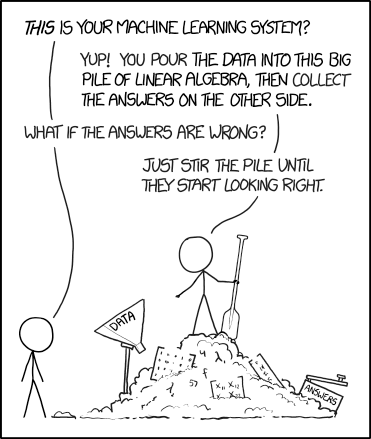
\includegraphics[scale=.4]{machine_learning}
        \end{figure}
    \end{columns}
    \addreference{\href{https://imgs.xkcd.com/comics/machine\_learning.png}{https://imgs.xkcd.com/comics/machine\_learning.png}}
\end{frame}

\begin{frame}{data}{insufficient data}
    \question{insufficient data in music}
    
    %\bigskip
    \begin{columns}
    \column{.6\linewidth}
    \begin{itemize}
        \item<1->   \textbf{music data} itself is not scarce (although there might be copyright issues...)
        \bigskip
        \item<2->   \textbf{consumer annotations} are more difficult to collect, but there are some large collections
        \bigskip
        \item<3->   \textbf{detailed musical annotations} are hard to come by, because
        \begin{itemize}
            \item   time consuming \& tedious annotation process
            \item   experts needed for annotations
        \end{itemize}
    \end{itemize}
    \column{.4\linewidth}
    %\vspace{-2mm}
    \begin{figure}
        
\includegraphics[scale=.1]{musicdata}
    \end{figure}
    \end{columns}
\end{frame}

\begin{frame}{data}{previous work on insufficient data}
	    \begin{itemize}
        \item   literature proposes many ways of \textbf{dealing with insufficient data}
            \begin{itemize}
                \item   data synthesis
                \smallskip
								\item   data augmentation\only<1>{\footfullcite{qin_tuning_2019}}
                \smallskip
								\item<2->   transfer learning\only<2>{\footfullcite{gururani_attention_2019}}
                \smallskip
								\item<3->   semi- and self-supervised approaches\only<3>{\footfullcite{wu_automatic_2017}\footfullcite{gururani_semi-supervised_2021}} 
                \smallskip
								\item<3->   \ldots
            \end{itemize}
			\end{itemize}
\end{frame}
